%% $RCSfile: proj_report_outline.tex,v $
%% $Revision: 1.3 $
%% $Date: 2016/06/10 03:41:54 $
%% $Author: kevin $

\documentclass[11pt
              , a4paper
              , twoside
              , openright
              ]{report}


\usepackage{float} % lets you have non-floating floats

\usepackage{url} % for typesetting urls

\usepackage{pdfpages} % for adding pdf

\usepackage{graphicx} % for adding graphics

\usepackage{appendix} % for using appendix

\usepackage{url}



%
%  We don't want figures to float so we define
%
\newfloat{fig}{thp}{lof}[chapter]
\floatname{fig}{Figure}

%% These are standard LaTeX definitions for the document
%%                            
\title{Why Do Programmers Do What They Do? \protect\\ A Theory of Influences on Security Practices}
\author{Lavanya Sajwan}

%% This file can be used for creating a wide range of reports
%%  across various Schools
%%
%% Set up some things, mostly for the front page, for your specific document
%
% Current options are:
% [ecs|msor|sms]          Which school you are in.
%                         (msor option retained for reproducing old data)
% [bschonscomp|mcompsci]  Which degree you are doing
%                          You can also specify any other degree by name
%                          (see below)
% [font|image]            Use a font or an image for the VUW logo
%                          The font option will only work on ECS systems
%
\usepackage[image,ecs]{vuwproject}

% You should specifiy your supervisor here with
%     \supervisor{Firstname Lastname}
% use \supervisors if there is more than one supervisor
\supervisors{James Noble, Craig Anslow}

% Unless you've used the bschonscomp or mcompsci
%  options above use
%   \otherdegree{OTHER DEGREE OR DIPLOMA NAME}
% here to specify degree
\otherdegree{Bachelor of Engineering with Honours in Software Engineering}

% Comment this out if you want the date printed.
\date{}

\begin{document}

% Make the page numbering roman, until after the contents, etc.
\frontmatter

%%%%%%%%%%%%%%%%%%%%%%%%%%%%%%%%%%%%%%%%%%%%%%%%%%%%%%%

%%%%%%%%%%%%%%%%%%%%%%%%%%%%%%%%%%%%%%%%%%%%%%%%%%%%%%%

\begin{abstract}

Technologies are continually adapting to match ever-changing trends, and as this occurs, new vulnerabilities are exploited by malignant attackers and can cause significant economic damage to companies. Programmers are therefore repeatedly having to expand knowledge and skills to protect software. Programmers do make mistakes, and this is why we must understand the thinking behind the decisions and influences of programmers to interpret how they implement and adopt security practices. Understanding these decisions can help inform design decisions around improving programming language security. This preliminary report will cover the current progress of the project "Why Do Programmers Do What They Do?"

\end{abstract}

%%%%%%%%%%%%%%%%%%%%%%%%%%%%%%%%%%%%%%%%%%%%%%%%%%%%%%%

\maketitle

\chapter*{Acknowledgements}\label{C:Acknowledge}

I want to thank my supervisors James Noble and Craig Anslow, for their ongoing support and direction as I have completed this project.
\newline
\newline
To dad and mum, thanks for harassing friends to potentially participate in this study. To dad, mum and Saumya, thank you all for having no idea about what I have been doing all year long, but for also leaving me relatively alone for these last weeks as I write, write, write and write. 
\newline
\newline
And to Janaye; a massive thanks for reading over this report and being my grammar and punctuation whizz since high school.

\tableofcontents

% we want a list of the figures we defined
% \listof{fig}{Figures}

%%%%%%%%%%%%%%%%%%%%%%%%%%%%%%%%%%%%%%%%%%%%%%%%%%%%%%%

\mainmatter

%%%%%%%%%%%%%%%%%%%%%%%%%%%%%%%%%%%%%%%%%%%%%%%%%%%%%%%

% individual chapters included here
\chapter{Introduction}\label{C:intro}

\par As software is now ubiquitous across industry and it is impossible not to have a presence in the tech sphere. Consequently, software security has become so significant, programmers have to ensure that the security processes that they implement are resilient to any attacks. Lack of attack prevention can cause leakage of sensitive information, massive economic damage and danger to massive numbers of users and employees, consequently opening business, clients and end-users to exploitation by external bodies. Unfortunately, every day, we hear of organisations that have been compromised \cite{1}. Last year New Zealand experienced a significant security breach within the Tū Ora Compass Health (Tū Ora) Primary Health Organisation (PHO) \cite{incident}. Tū Ora is one of the largest PHO's in the country and it governs the greater Wellington region \cite{incident}. Personal information of up to one million New Zealander's was exposed and the effects of this are ongoing \cite{incident}. Ccosts have been great in attempts to mitigate any effects to the public. Dedicated call centres have had to be organised as well as dedicated mental health lines \cite{healthpol, incident}. Regular updates have had to be released in order to maintain communication transparency and assurance quality measures are ongoing \cite{healthpol, incident}.  
\newline
\par Qualitative research is often neglected and overlooked in favour of more quantitative reasoning and technical traits such as the security method used or the programmers task-completion rate \cite{3}. Programmers provide a human aspect to a technical solution and therefore, there should be a shift towards understanding the more background ‘soft’ processes that occur when making decisions; why are the choices made based on past influences, and how they affect the programmers work in the present? 
\newline
\par Past the research aspect, when security and privacy issues do occur in real-world scenarios, developers are blamed first as it is their projects that have allowed the vulnerabilities to be exploited \cite{4}. While developers do make mistakes, they also do need the support to make better security decisions, and this support is currently lacking in the industry \cite{4}. Education is limited past initial acceptance within organisations, and often developers have a blasé attitude to the matter expecting another team to fix the issue \cite{5}. Furthermore, security mechanisms often have an increased complexity, which make them difficult to understand and to then use \cite{6}.
\newline
\par This project will investigate how software developers implement and adopt security practices in the work they do in order to develop an understanding of what influences and impact decisions surrounding their technical work. This project will be conducted using grounded theory which is a theory is a method which aims to establish a theory when there is none \cite{2}, and it is a commonly used method for data analysis. Interviews will take place to collect the data, from which the answers will be analysed to draw conclusions on standard security practices in the professional workplace. This project builds upon works by Hala Assal, Charles Weir and Nathan Newton \cite{summary1, 1, nathan}. 
\newline
\par This project aims to implement a theory as to why programmers implement and adopt security practices in the work they do by interviewing professional developers and using the Grounded Theory Method to analyse the outcomes. Grounded theory is a research method to analyse qualitative data. There are several thorough steps which include; sampling, data collection, data analysis, theoretical note writing, identifying core categories, forming theoretical outlines and presenting a theory.
\newline
\par Participants will be recruited by posting on tech-related groups (i.e. From OWASP Meetup Group and LinkedIn) and mailing lists and also using mine and my supervisor contacts. At this point, I can then start semi-structured interviews with 10-20 interested individuals on their security practices while programming. These people will all be developers in New Zealand that are in varying stages of their careers and career paths to allow for a broader range of responses and a case study relevant to New Zealand. Examples of appropriate job titles include; DevOps engineer, front-end security developer, database administrator, developer, programmer and security architect.
\newline
\par This project will lead to a new, more in-depth understanding of the psychology of the decisions made by programmers. The research done by this project could lead to future qualitative research to be done on another under-developed topic on why programmers do what they do. Paired with this research, that future one could help build a profile of a programmer and their thought processes. Data collected could also be the foundation that allows a developer to build tools that helps other developers implement proper security practices; a Grammarly for security. It can also help the further development of existing static analysis tools such as Infer developed by Facebook, Tricorder used by Google, Coverity and Raygun \cite{infer, tri, coverity, raygun}. These tools all work by providing security detection modules and are used for quality assurance and security. 
\newline
\par Exploring this topic is essential as it allows for a more comprehensive understanding of how and why programmers think the way they do, and of the human and social aspects of Software Engineering \cite{geeks}. We want to understand what solutions developers are using to implement in their security practices, if at all. The findings from this can support developers in terms of education and the better design of security methods in programming \cite{summary1} that have an emphasis on usability. The findings of this project can also be used to identify what security methods developers find as beneficial in their programming. This will allow programmers to complete their work to a high standard, by adhering to proper security protocols, thus overall making their work of a higher value both in a secure and professional sense.

\section{Deviations from the Original Plan}
There have been no deviations from the original plan.
\chapter{Background}\label{C:Background}

\par Conceptually, this project aims to gather data in order to ultimately form a theory. Therefore, It is essential that I know enough information about the topic of security so that I am able to interview professional engineers in a manner which is knowledgeable. This chapter will include background on the importance of information security practices, what practices are widely used, and summaries on existing research on similar subject matter. 

\chapter{Work Completed}\label{C:Completed}

\par As of yet, the progress made on this study has been predominately focused on the human ethics application as well as the steps in crafting appropriate interview questions. Before any contact with potential interview participants, the human ethics application has to be approved. This is to ensure that research follows responsible and robust processes involving people and their data, consequently, proceeding ethically. As this has been in a recursive stage of editing and sending back to be reviewed, there has been iterative work designing potential questions for the semi-structured interview. Processes which have involved pilot studies in order to focus on an area of my topic. As the human ethics application is yet to be approved, my data collection and analysis stages have not started. Each of the areas are discussed in detail in the following sections. 

\section{Human Ethics Application}

\par There was an immediate pressure to complete the human ethics application as the rest of the project is highly dependent on the participant interviews. This meant that the research had to be planned quite quickly in order to provide the human ethics committee with all the relevant information needed to approve the application. The initial application was submitted 8th of April. It has since undergone pre-committee revisions and post-committee revisions and is currently pending a second committee review. This application outlined a series of multichoice and short-answer questions which had to be answered thoroughly and supporting documents had to be submitted. These supporting documents included the participant information sheet, consent to interview document, an interview guide, and as this research’s recruitment will be done through mailing lists and Meetup and LinkedIn posts, a sample recruitment post was also supplied. 
\newline
\par The human ethics application specified key methods for ethical data collection in order to maintain a research that followed ideal  human ethics policy
(https://www.wgtn.ac.nz/documents/policy/research-policy/human-ethics-policy.pdf
). The application went into details of data collection and recruitment, conformation with the university Te Tiriti o Waitangi statute, project risks, and data management. Answering these sections meant that a lot of planning has gone into the interview process for data collection. In particular it was decided that the selection process will follow purposeful sampling for the interviews. This is because participants will need to be selected on whether they are professional programmers in industry. The study will ideally include participants with a range of job titles and years in the field in order to find interesting comparisons during the interview process in the way security practices are adopted in the developed software. Participants will consequently be filtered by appropriate job titles, and be older by the age of 18 to avoid complexities with the Vulnerable Children Act 2014
\textbf{(http://www.legislation.govt.nz/act/public/2014/0040/latest/DLM5501618.html?src=qs
)}. 
\newline
\par Focus on the Te Tiriti o Waitangi was necessary as this is a research project run in New Zealand with participants who work in the domestic industry. Therefore, the recruitment of participants and the conducting of the interviews will be run in a way which respects the principles outline in the university statute, which derive directly from Te Tiriti o Waitangi. Specific care was taken to this as there is only a certain threshold that this study can pertain to. However, it was decided that through my recruitment, I should work under the principle of Whai wāhi (participation) and encourage the participation of tangata whenua by advertising it on accessible platforms and to organisations with more of an emphasis of Te Tiriti in their core values. An alum of Maori decent was also consulted on this and they mentioned that in the participant information and consent forms, it should be explicitly clear that participants still have ownership of their data and are able to edit and remove information as they wish. 
\newline
\par Corresponding to the point above, the interviews will be confidential rather the anonymous to allow for participant emendations and to also allow for follow up questions if necessary. They will in no way be able to be identified and in any report outputs of this study will not name participants and instead be either referred to by role or by pseudonyms. Data will also be aggregated to maintain confidentiality. Participants will also be reminded before the interview as well as in the information and consent documents, that they should not divulge any sensitive information. 
\newline
\par Due to complications with COVID-19 the interview will also be adapted to allow for online capabilities using applications such as Zoom. There were issues surrounding obtaining consent, and the application had to be amended to allow for electronic consent. This will be done by emailing the form to participants, and consent will be obtained by a simple email back of agreement. Electronic signing of the form was not applicable as not everyone may have access to software with the capabilities to do so. It was also decided that the interview will offer a gift reward for participation for their time during the pandemic and this will be a supermarket voucher. Safety was consequently paramount in the planning of the pandemic for both the interviewer and the interviewee. In the case of any in-person interviews sanitiser and a box of tissues will be in hand as well as disinfection of the meeting rooms before and after interviews, and the interviews themselves will be conducted while maintaining social distancing practices. To thank participants for their time, they will be offered a gift voucher to a supermarket.



\section{Interview Planning}

\par In the ethics application planning had to occur well ahead of interviews and there was a focus on creating the questions. However, as grounded theory involves a semi-structured interview process, a guide was submitted alongside the application. This is because questions are meant to change dependent on the participant as well as the narrowing focus on the ultimate theory. The interviews will also include open-ended questions which allow for more personal, in-depth responses which can hold more information to be analysed. It is expected that the analysis will occur immediately after interviews in order to revise questions before the next participant.  All interviews are expected to take a minimum of 30 minutes, and will be transcribed. This transcription will be available for participants at their request for any amending of content.
\newline
\par Interviews will be expected to start by collecting information on participant background. This means groupings can happen by education, roles and experience. The next section of the interview will cover their current security practices that they implement in their code. This will then lead on to the impacts of security and languages in the projects they have worked on, and any background in the testing of those practices and successes of some over others. These sections allow for the simplest of aggregations to occur when all data has been collected and analysed. 
\newline
\par For a better understanding of the process, old alums whom conducted grounded theory methodology studies were contacted on their approaches. One stated that they did not know what their focus would be going into the interviews, and the idea slowly formed the more interviews and analysis he did. The other stated that they was almost “over-prepared” in the sense that they had read many academic articles that none of the industry members knew specifics about. Both had the similarities that going into the interview stage, they had very broad questions that did not quite relate to each other. Those questions did not encourage the high-ended answers this study promotes. 
\newline
\par Potential interview questions have been planned alongside these sections. However, much like the issues with the alums, they are too broad and are disjointed of each other; often focusing on several different aspects of security practices. More thought is going into these questions to having a specific focus, which will provide the semi-structured interview the flow it needs to collect concise data.


\section{Pilot Study}

\par After obtaining relevant feedback on the questions, a suggestion was made to run a small pilot study.  The objective of a pilot study is to enhance the likelihood of success in the main study and to avoid any risks to completion
\textbf{https://www.ncbi.nlm.nih.gov/pmc/articles/PMC2824145/}
. The first pilot study conducted was to provide evidence on the level of efficiency of the outlined potential interview questions. The efficiency being that of the potential to obtain open answers with a ultimate focus in mind. This focus will allow for more detailed answers which can be analysed to draw closer comparisons to form a stronger theory. The participant of the pilot study was another alum of the university and a personal contact. This pilot solidified that the potential questions are definitely too broad in scope. It was also highlighted that a few questions were quite similar and can be condensed. The questions were also not as opened-ended as desired, which made the answers seem not very valuable. As this pilot study was about testing the questions the participant of the pilot study was asked every question. This meant that this interview did not follow a typical grounded theory approach in which questions are asked dependent on the participant. 
\newline
\par For the following pilot interview, this was not an issue as with more clarity on questions. Therefore the typical grounded theory approach to interviews was followed and questions were dependent on the interviewee. The person being another personal contact. More concise questions were asked, but from this second interview, it is apparent that the questions need to be written in a way that promotes discussion. As an interviewer, there also needs to be more practice in continuing the conversation and adapting questions to the last answer. 

\section{Advertising}

\par The study will need to be advertised through mailing lists and websites like Meetup and LinkedIn. A recruitment post has been made for this as well as the support of a simple web-page to present this study as professional and legitimate – traits especially important to programmers interested in security practices. The advertising has not been released yet as the human ethics application is still pending approval. However, as everything has been planned and ready, as soon as the approval has been made, recruitment can begin. 
\newline
\par Following the principle of Whai wāhi, the recruitment posts and web-page include the use of Te Reo. This is simple way of respecting tangata whenua, but is also more welcoming towards any potential Maori participants.








\chapter{Future Work}\label{C:future}

\par This section outlines the remaining work to do for the completion and evaluation of this project. It will also provide a proposed timeline in which this will happen. 

\section{Work Remaining}

\par The work completed this semester has laid the foundations to start work on the formal investigation as soon as the human ethics application is approved. The work remaining consists of outlining some more relevant interview questions, conducting interviews and analysing answers to find an overarching theory.
\newline
\par Defining relevant interview questions has been partially completed. By outlining sections in the interview guide that was submitted with the human ethics application the topics that the questions should fall under are known. After pilot testing there has been a better understanding of the types of questions to ask. Next steps for writing potential questions are to develop them into questions which focus on a specific topic, while also making sure they feature a majority of open-ended questions. These types of questions will motivate the participants to give longer and more concise responses which will allow for patterns to form when analysing the answers.
\newline
\par When the human ethics application is approved sampling can occur. As the recruitment methods have all been finalised, all that needs to be done is posting of the relevant information on mailing lists, Meetup and LinkedIn groups, and also using my own connections. They will be selectively chosen dependent on their role titles and other diversifying factors in order to find patterns across groups of people consequently avoiding any biases. It is important that recruitment occurs through different mediums, as it is not always that everyone will be interested in participating – especially with a topic related to security.  Sampling then leads onto data collection.
\newline
\par The form of data collection for this study is through interviews. They will be recorded to allow for focus to be on the participant and to mitigate a flow of conversation. This allows to concentration to be evenly distributed through the different steps of study. The interview will be semi-structured to allow for evolution in the questions \cite{geeks}. 
\newline
\par Analysis will occur after each interview. This process will use open coding to analyse key points from the interview transcript \cite{geeks}. Open coding is the process of keeping the mind free from any biases when sorting information. This means any assumptions should be ignored and ideas can only form from the data collected. This part of the remaining work is expected to take the longest. When concepts are identified these can influence the iterative nature of the interview and allow for the following interview to perhaps have different questions, target towards the found concepts. After the interviews and their following analysis, the core categories are found and then the theory can be presented in the final report and presentation. 
\newline
\par 
There are limitations to evaluating the solution as the project does not produce a technical artefact. Pertaining to the method; there are two significant areas of evaluation that can be taken. These are the evaluation of the research process and theory and will occur after the generation of the final theory. By evaluating these two areas, it can be examined whether correct procedures have taken place, and determine whether project goals have been met.
 
\section{Proposed Timeline}

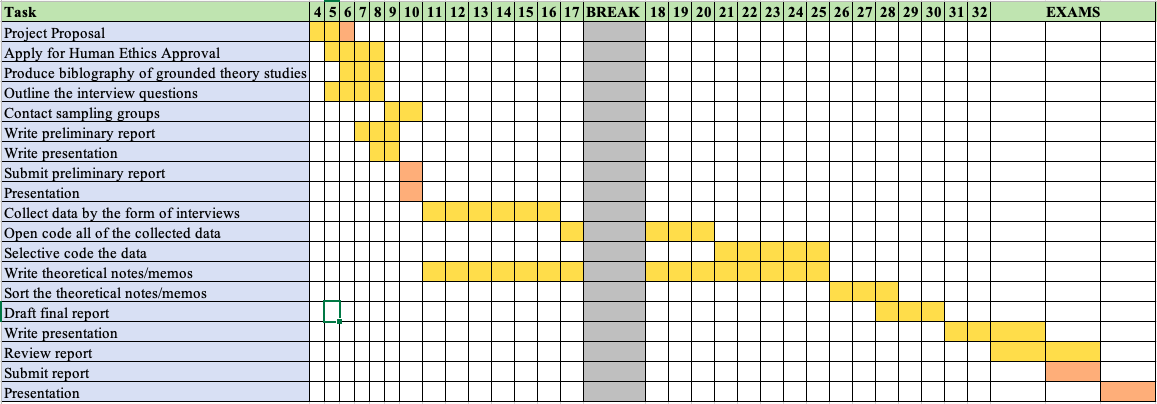
\includegraphics[width=\textwidth]{figures/fig1.png}
\newline
\newline
Above shows the Gantt chart which was outlined during the submission of the proposal. This outlined the timeline that the project would follow and what deadlines would fall within this course. 
\newline
\newline
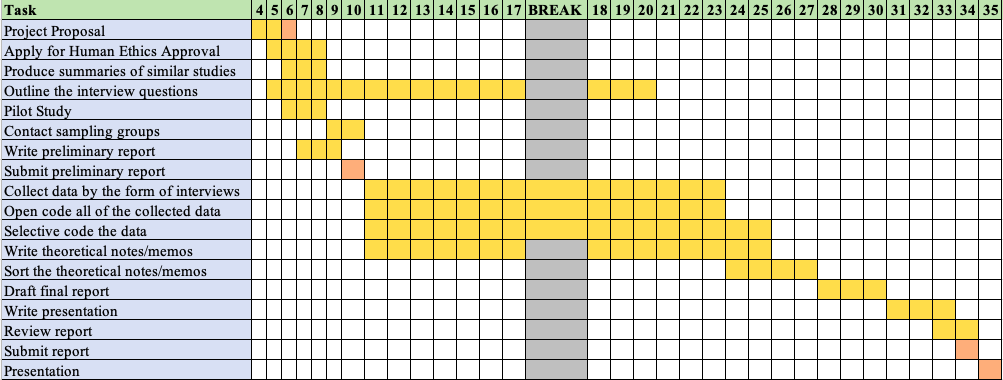
\includegraphics[width=\textwidth]{figures/fig2.png}
\newline
\newline
The above shows the now amended timeline. Not much has changed as I am following the proposed timeline quite closely. There have been additions of a pilot study which ran across weeks 6 and 7. There are still details awaiting regarding the examination period in semester two so the “EXAM” columns are amended to being week columns. The initial analysis stage of this research has also been pulled back to starting alongside the interview process as analysis will ideally occur after each interview. The entire timeline is dependent on whether the human ethics application obtains approval by the end of week 10. if this does not occur, the entire timeline will have to shift back and tasks may have to be condensed.







\chapter{Feedback}\label{C:feedback}

Feedback on what would be an interesting area of focus would be much appreciated. I am currently focusing on education, but that almost seems like a overdone field. However, it is something of interest to me, so perhaps any input on how to make it more unique. Any feedback on the potential questions and one how to adapt questions to participants will also be much appreciated. Overall, interview and grounded theory feedback would also be helpful. 


%%%%%%%%%%%%%%%%%%%%%%%%%%%%%%%%%%%%%%%%%%%%%%%%%%%%%%%

\backmatter

%%%%%%%%%%%%%%%%%%%%%%%%%%%%%%%%%%%%%%%%%%%%%%%%%%%%%%%


%\bibliographystyle{ieeetr}/acm
\bibliography{6-references}
\bibliographystyle{ieeetr}

% appendix
\appendix
\chapter{Proposal}

\includegraphics[height=0.8\textheight]{appendix/proposal.pdf}

\includepdf[pagecommand={\thispagestyle{plain}}, pages={2-last},scale=0.8]{appendix/proposal.pdf}
\chapter{Application}
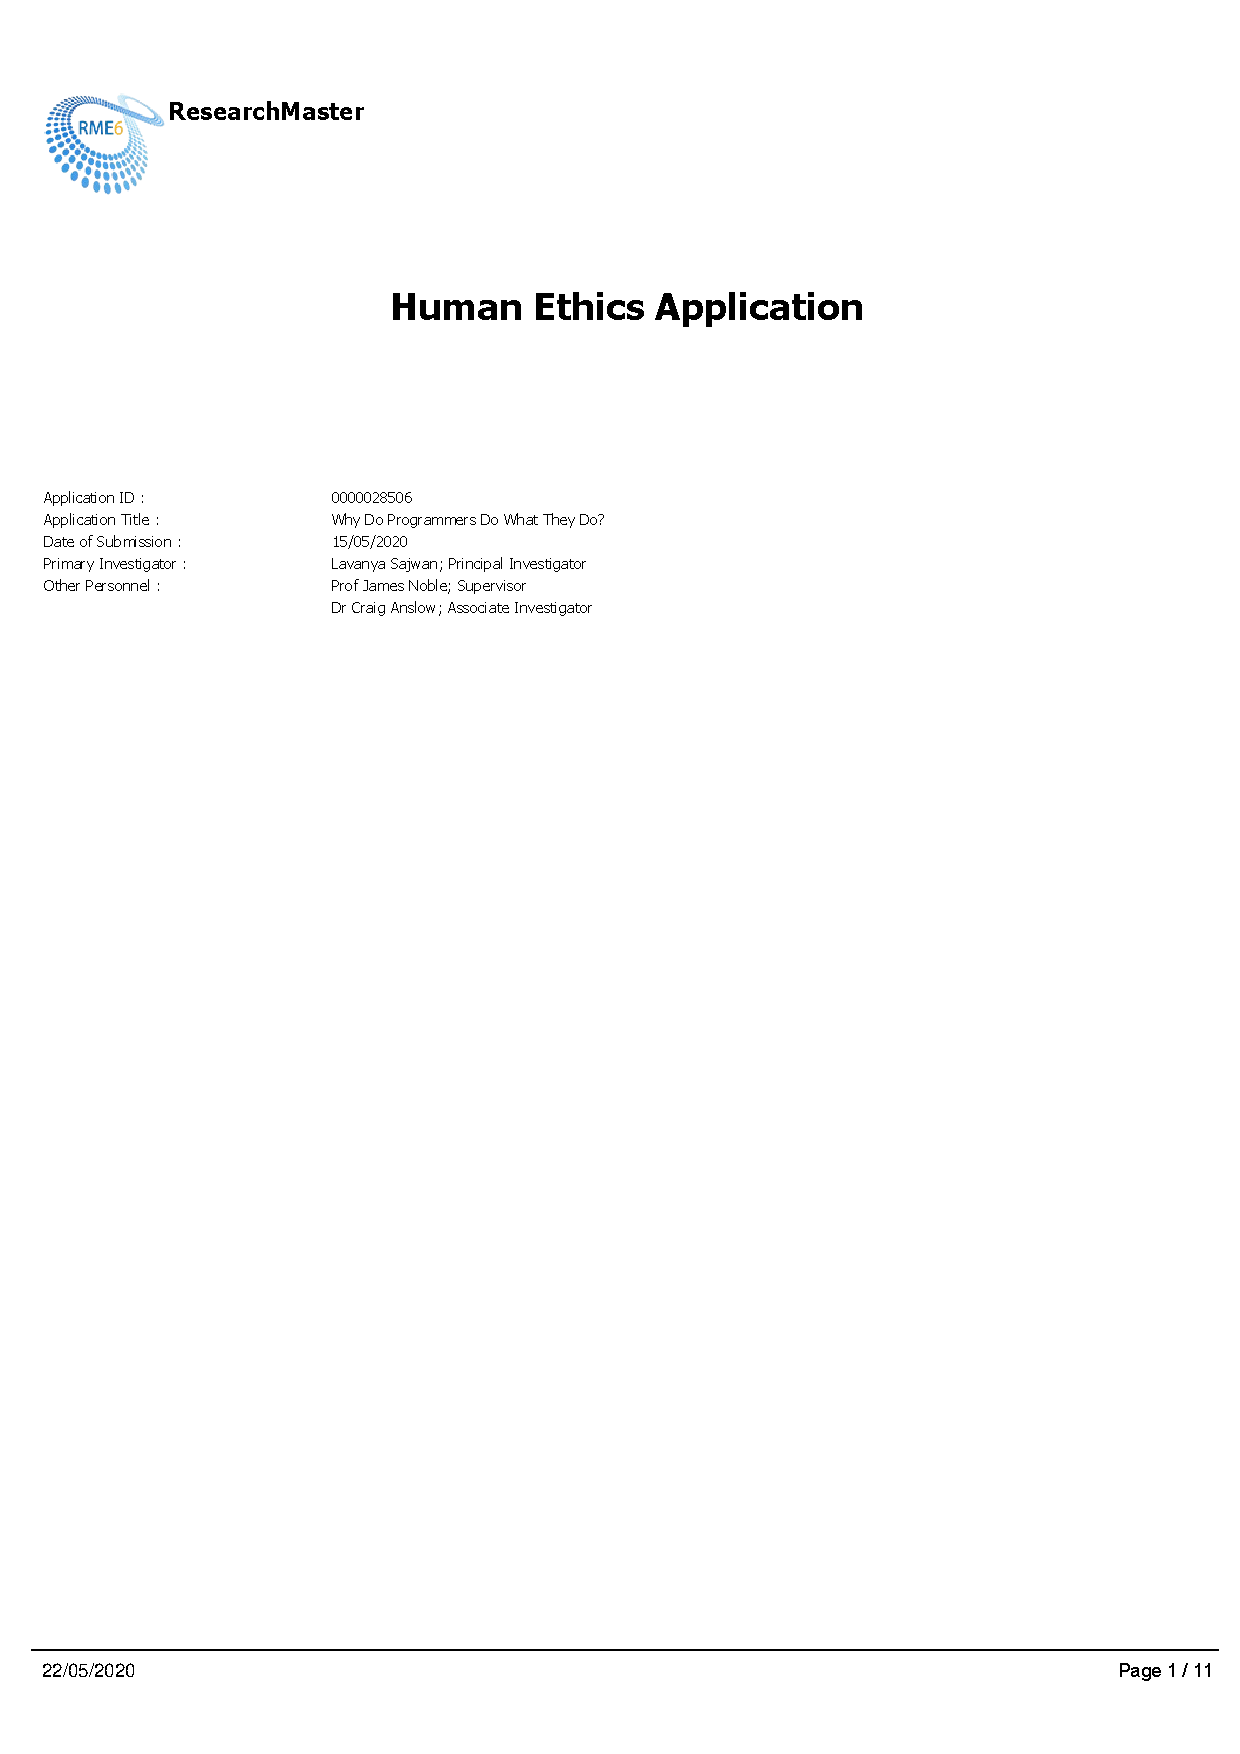
\includegraphics[height=0.8\textheight]{appendix/humanethics.pdf}
\includepdf[pagecommand={\thispagestyle{plain}}, pages={2-last},scale=0.8]{appendix/humanethics.pdf}





\chapter{Participant Information Sheet}
\includegraphics[height=0.8\textheight]{\string"Participant_Information_Sheet".pdf}

\includepdf[pagecommand={\thispagestyle{plain}}, pages={2-last},scale=0.8]{Participant_Information_Sheet.pdf}


\chapter{Participant Consent Form}

\includegraphics[height=0.8\textheight]{appendix/consent.pdf}

\includepdf[pagecommand={\thispagestyle{plain}}, pages={2-last},scale=0.8]{appendix/consent.pdf}


\chapter{Interview Guide}
\includegraphics[height=0.8\textheight]{\string"Interview_Guide".pdf}

\includepdf[pagecommand={\thispagestyle{plain}}, pages={2-last},scale=0.8]{Interview_Guide.pdf}


\chapter{Recruitment Post}

\includegraphics[height=0.8\textheight]{appendix/post.pdf}
\chapter{Recruitment Webpage}
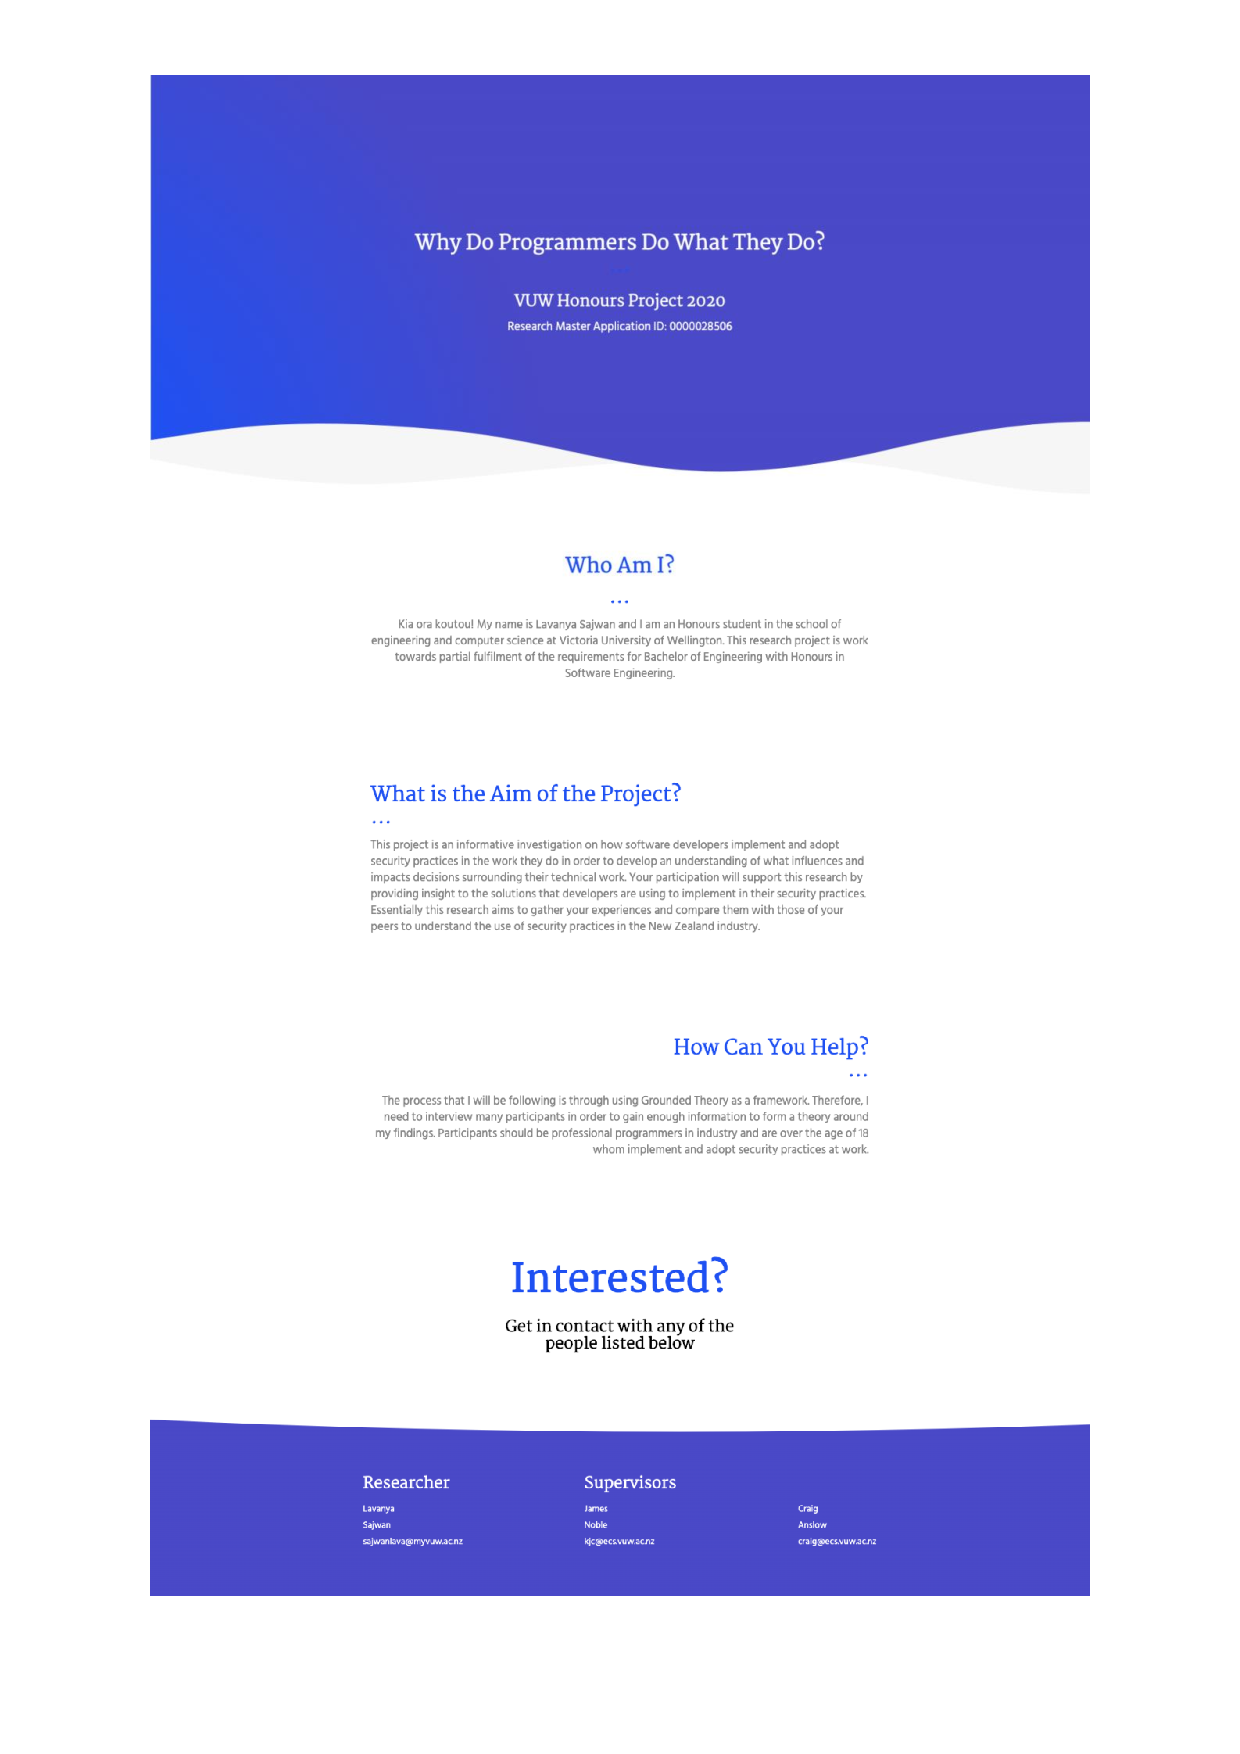
\includegraphics[width=\textwidth]{appendix/webpage.pdf}
\chapter{Initial Interview Questions}
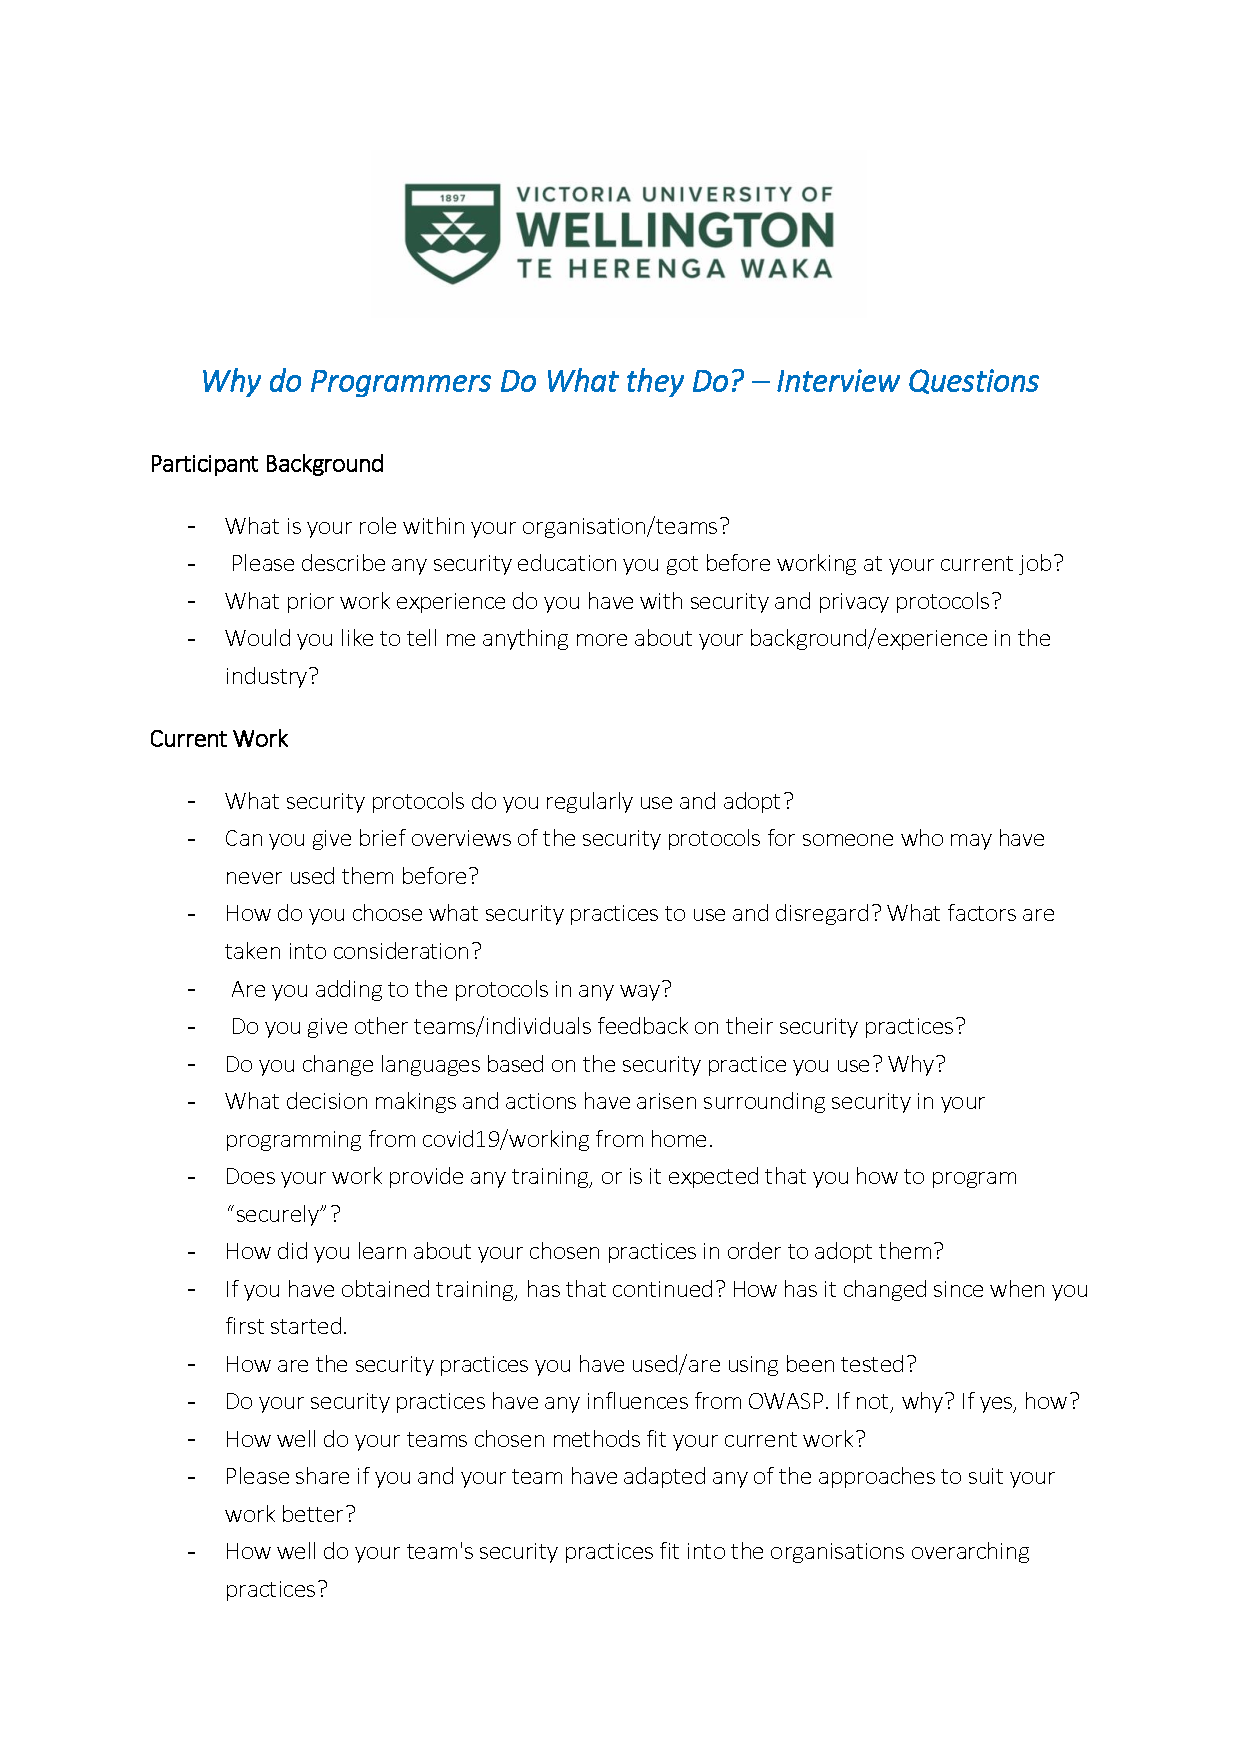
\includegraphics[height=0.8\textheight]{appendix/pilot1_questions.pdf}
\includepdf[pagecommand={\thispagestyle{plain}}, pages={2-last},scale=0.8]{appendix/pilot1_questions.pdf}


\end{document}
